\section{Discussion} 
\todo{the decision to annotate text using the VAD structure was maybe a limitation, other structures could be looked into further?}

\subsection{How can textual sentiment prediction be optimised?}

Two main methods of predicting the sentiment of input text have been analysed, using a bag-of-words method, and using machine learning approaches.

The lexicon based bag-of-words is based entirely on having an appropriate dataset to rank the words, since as Table \ref{lexicon:f1} shows, having rated VAD scores which follow a certain structure is key to obtaining good results. Dimensions like the Dominance and Arousal of a piece of text can be very subjective, and vary depending on what the data is ranging these scores from. 

The decision to use the machine learning based model for the implementation is due to having overall more stable F1 scores for each dimension, but this is only due to training and testing over the same dataset. 

One point which has not been addressed by this investigation is that the VAD values for each sentence are related to one another. This can be shown by the mosaic plot of the data in Figure \ref{mosaic:emo}, where we can see that the majority of the data is taken up by samples which are neutral in all three dimensions, IE. \todo{is this correct?} if the prediction over a sentence returns that it has neutral Valence and Arousal, then it is much more likely to have a neutral Dominance. Figure \ref{mosaic:emo} also displays the Pearson residuals for the data, which shows that for many of the classes that contain Neutral values, particularly neutral Arousal there are a lot less samples than expected when a Pearson $\chi^2$ test is performed comparing to the null model if the values were not related. This test was as it tests against a null hypothesis that the distribution of values are independent, and in this case it rejects this null hypothesis with a p-value of 2.22E-16 \cite{zeileis2007residual}.

\begin{figure}[ht]
\centering
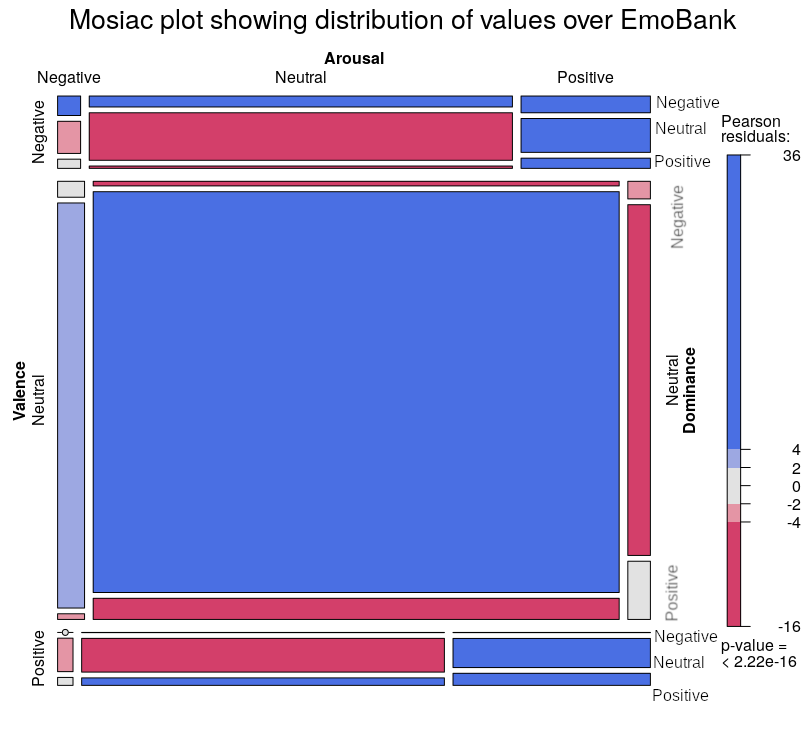
\includegraphics[scale=0.7]{graphs/mosaic_new.png}
\label{mosaic:emo}
\caption{Emobank data distribution with relationships. The Pearson residuals are the deviation from the expected frequency by a Pearson $\chi^2$ Test \cite{pearson1900x}}
\end{figure}

Because of this, a small extention investigation was done using the existing model setup as given in Section \ref{finalModelSection} to train a model to each predict a V, A, D value, given the other two as inputs, as shown in Figure \ref{model:adjust}. Since these adjustment models do not take in the input sentence, the number of feature selection and n-gram values were not needed. Ideally, a model would be trained off all the values 

\begin{figure}[ht]
\centering
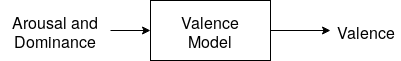
\includegraphics[scale=0.6]{implementation/adjustModel.png}
\label{model:adjust}
\caption{Diagram showing inputs and outputs for the valence prediction model}
\end{figure}

These models have good F1 scores compared to the model with the sentence data, and more investigation needs to be done on how to incorporate these adjustment models into the final result. For a quick prototype of implementing this, the decision was made to make a small adjustment to the score given back by the main prediction model. The values that it was chosen are relatively arbitrary and further work could be done to investigate the optimal way to handle the dependency of these variables further.


\begin{table}[h]
\centering
\caption{F1 scores for adjustment models}
\begin{tabular}{|l|l|}
\hline
Model & F1 Score \\ \hline
 Valence Prediction &  0.778\\
 Arousal Prediction &  0.864\\
 Dominance Prediction &  0.893\\
 \hline
\end{tabular}
\label{f1:adj}
\end{table}

\subsection{Does using more than 1 dimension to classify emotions provide more insight, and how can this be quantified?}



To be able to evoke enough emotive text from a user, the UI states "Please describe how your week is going so far. Be as detailed as possible.". This was arbitrarily chosen as just a question that does not simply have a yes or no answer, and an investigation could be made in future to find a better way of inspiring the optimal amount of input text an particularly emotive style.

All but 2 of the tests gave the result Ekman's emotion back as "Surprise", and the other two came back with "Disgust" which was incorrect every time. An explanation for this results would be because, as shown in \todo{contintue}


\subsection{Project Reflection and Future Work}

\todo{Choosing how to relate the VAD values to the data returned for the songs is relatively arbitrary and something that if there was more time could be investigated further.}
